% \part{Implementation}

\section{Method}

To implemented the proposed system, we divide the system into three main parts: head tracking, 3D effect, and curved display corrention. In Section4.1, we introduce the basic structure of algorithm and the intra-process communication framework used. Section4.2 introduced head tracking part, which is responsible for tracking the user's head movement and providing the user head's position and do filter. Section4.4 introduce methods and details about how to implement 3D effect, including unity simulation part and off-axis projection implementation. Section4.4 introduce the curved display correction, which is responsible for correcting the image distortion on the curved display.

\subsection{Framework}
System's framework can be devided into two parts in platform level: C++ level and Unity level. C++ level is responsible for head tracking and image correction, and Unity level is responsible for off-axis projection and simulation constructing. The communication between C++ and Unity is based on Robot Operating System 2(ROS2)\cite{ros2} and Unity's ROS2 plugin\cite{ros2forunity}, since ros2 provided a convinience way to both communication and data visualization.

% \begin{figure}[htb]
%     \centering
%     \includegraphics[width=0.5\textwidth]{example-image-a}
%     \caption{Code structure and working-flow}\label{F:test-a}
% \end{figure}

In detector, we use YuNet\cite{Wu_2023} to detect the user's face and get the face's key points. Then keypoints is sent to pnp solver, which return head's position in camera frame and send to tracker. Tracker node process head's position, applying CV motion model to kalman filter and send result to Unity part. In Unity, we have constructed a simulation environment, which include two position-synchronized cameras to simulate the movement combination of rendering camera and human head. Render result will be sent to wrap node, which apply finally image correction and send to display.

To achieve a sufficiently immersive effect, it is essential to:
\begin{itemize}
    \item Ensure a stable head position to prevent the resultant image from shaking.
    \item Minimize system processing time to enable fast response in real-time 3D systems.
    \item Provide reliable image correction to prevent distortion on curved displays.
\end{itemize}

\subsection{Head Tracking}
In head tracking part, we use YuNet\cite{Wu_2023} to detect the user's face and get the face's key points, and applying CV motion model to do filter.

\subsubsection{Detector and Locator}
OpenCV 4.5.4\cite{opencv_4_5_4} have integrated YuNet as one of face landmark detection function. \footnote[1]{Onnx model file can be found at \href{https://github.com/opencv/opencv_zoo/tree/main/models/face_detection_yunet}{OpenCV Model Zoo}}

% \begin{figure}[htb]
%     \centering
%     \includegraphics[width=0.5\textwidth]{example-image-a}
%     \caption{YuNet network structure}\label{F:test-a}
% \end{figure}

In OpenCV's API, YuNet accept a RGB image as input, and return a n * 14 size matrix, while n is the number of faces detected in the image. For each row, the first 4 elements are the bounding box of the face, and the rest 10 elements are the key points of the face, representing right eye, left eye, nose, right chin and left chin.

% For localization, OpenCV also privide solvePnP() as a pnp solve api. Since solvePnP() function return camera's pose in world frame, we defined face-frame pnp's world frame(Figure 14).



For localization, OpenCV also provide solvePnP() as a pnp
 solve api, with input of 3d points(world frame), 2d points(opencv's image frame), camera matrix and distortion matrix as input, output of camera's pose in world frame. Since solvePnP() function return camera's pose in world frame, world frame is defineded same as face-frame. Figure 10 shows the face-frame definition.

\begin{figure}[htb]
    \centering
    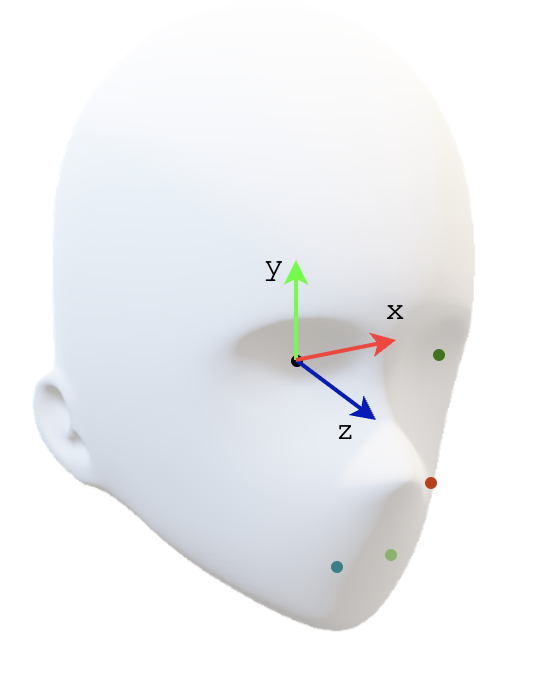
\includegraphics[width=0.5\textwidth]{figures/Preliminaries/faceFrame.png}
    \caption{Face-coordinate definition}\label{F:test-a}
\end{figure}

In addition, ePnP is chosen by its low-latency\cite{EPnP_2009}. Also, we've obtained camera's intrinsic matrix and distortion matrix by ros2 camera calibration package\cite{ros2_camera_calibration}, and applicated 3d-keypoints in a sample human head's model from Soheil M. etc(2023)'s work.\cite{soheil2023facial}

\subsubsection{Kalman Filter Design}
Consider the general movement of human head, we choose Kalman Filter as our motion model, since the head movement is a linear dynamic system. The state variables can be defined as head's:
$$
x_k = \begin{bmatrix} x & y & z & v_x & v_y & v_z \end{bmatrix}^T
$$

$$
z_k = \begin{bmatrix} x & y & z \end{bmatrix}^T
$$

while $x, y, z$ is the position of the head, and $v_x, v_y, v_z$ is the velocity of the head. 
Consider head's movement as a constant velocity(cv) model, the state transition equations can be defined as:
$$
\begin{cases}
    x' = x + v_{x} \cdot dt \\
    y' = y + v_{y} \cdot dt \\
    z' = z + v_{z} \cdot dt 
\end{cases}
$$
and observation equations:
$$
\begin{cases}
    x_m = x \\
    y_m = y \\
    z_m = z
\end{cases}
$$

while $x_m, y_m, z_m$ are variables in measurement space, and $dt$ is the time interval between two frames. 

In this case, we can generate the state transition matrix $F_k$ and measurement matrix $H_k$ as:

$$    
F_k = \begin{bmatrix} 1 & 0 & 0 & dt & 0 & 0 \\ 0 & 1 & 0 & 0 & dt & 0 \\ 0 & 0 & 1 & 0 & 0 & dt \\ 0 & 0 & 0 & 1 & 0 & 0 \\ 0 & 0 & 0 & 0 & 1 & 0 \\ 0 & 0 & 0 & 0 & 0 & 1 \end{bmatrix} 
$$
$$
H_k = \begin{bmatrix} 1 & 0 & 0 & 0 & 0 & 0 \\ 0 & 1 & 0 & 0 & 0 & 0 \\ 0 & 0 & 1 & 0 & 0 & 0 \end{bmatrix}
$$

By given the process noise covariance matrix $Q_k$ and measurement noise covariance matrix $R_k$ a proper value, we can apply Kalman Filter to track the head's position.

\subsubsection{Target Lost and Target Switch}
In most cases, tracking algorithm can works well and provide a reliable result. However, target lost will happen in minority of situation, since face landmark detector may fail or traking target switches, which may lead to an abnormal condition since filter will update its sta by a wrong measurement. To handle this condition, an additional threshold variable is set to determine whether the measurement position is reliable. For each frame, the predict step and update step of kalman filter is divided, and the update step will only be executed when the measurement is close enough to the prediction, otherwise reset $x,y,z$ to prediction and $v_x,v_y,v_z$ to 0.


\subsection{Simulation}

The simulation part is developed in Unity, a responsible graphic engine which is widely used in film and game industry. Simulation environment is devided into two sub-parts: user part and render part.
\begin{itemize}
    \item \textbf{User Part}: contains one viewing camera object and one plane object. Viewing camera's transform is synchronized with user head's position by subscribe to tracker node with the support of ROS2ForUnity. Plane object is by a specific meterial, to display render result from render camera.
    \item \textbf{Render Part}: contains one render camera and some example objects. Render camera is processed by an off-axis projection matrix, and will motion is synchronized with viewing camera. Render camera will also publish result image by ros2 component for correction algorithm. Example objects are used to test the 3D effect.
\end{itemize}

% \begin{figure}[htb]
%     \centering
%     \includegraphics[width=0.5\textwidth]{example-image-a}
%     \caption{Simulation Environment Structure}\label{F:test-a}
% \end{figure}

Each steps are described as follows:
\begin{itemize}
    \item \textbf{Step 1}: Viewing camera receive head's position from tracker node, and update position.
    \item \textbf{Step 2}: Render camera take a motion, to adjust its position to simulate the user's head movement.
    \item \textbf{Step 3}: Camera rendering the scene with off-axis projection matrix, and publish it by publisher provided by its ros2 component.
    \item \textbf{Step 4}: Material in screen plane update, viewing camera publish the image as a ros topic to show the illusion when screen have no distortion.
\end{itemize}

Coordinate of these two part are also synchronized by two anchor points. Anchors performs as two parts coordinates' origin. By this way, objects in two parts can use same relative coordinates, and get a better performance when position synchronize.

\subsection{Curved Displays Correction}
According to the user's different three-dimensional coordinates in space, the visual effect of the screen shape changes accordingly. This technique only considers the horizontal deformation of the screen, referred to here as the visual angle. Define the center of the curved screen as the origin \( O(0,0) \), with point \( A \) on the left and point \( B \) on the right of the screen, the radius of curvature as \( r \), and the central angle of the curved screen as \( \beta \). The user's eye position in the two-dimensional coordinate system is \( N(a,b) \), and the number of equal divisions of the screen \( n \) (within a certain range, the larger the parameter \( n \), the better the visual effect). The user's current visual angle \( \alpha \) can be calculated as follows:

\begin{figure}[htb]
    \centering
    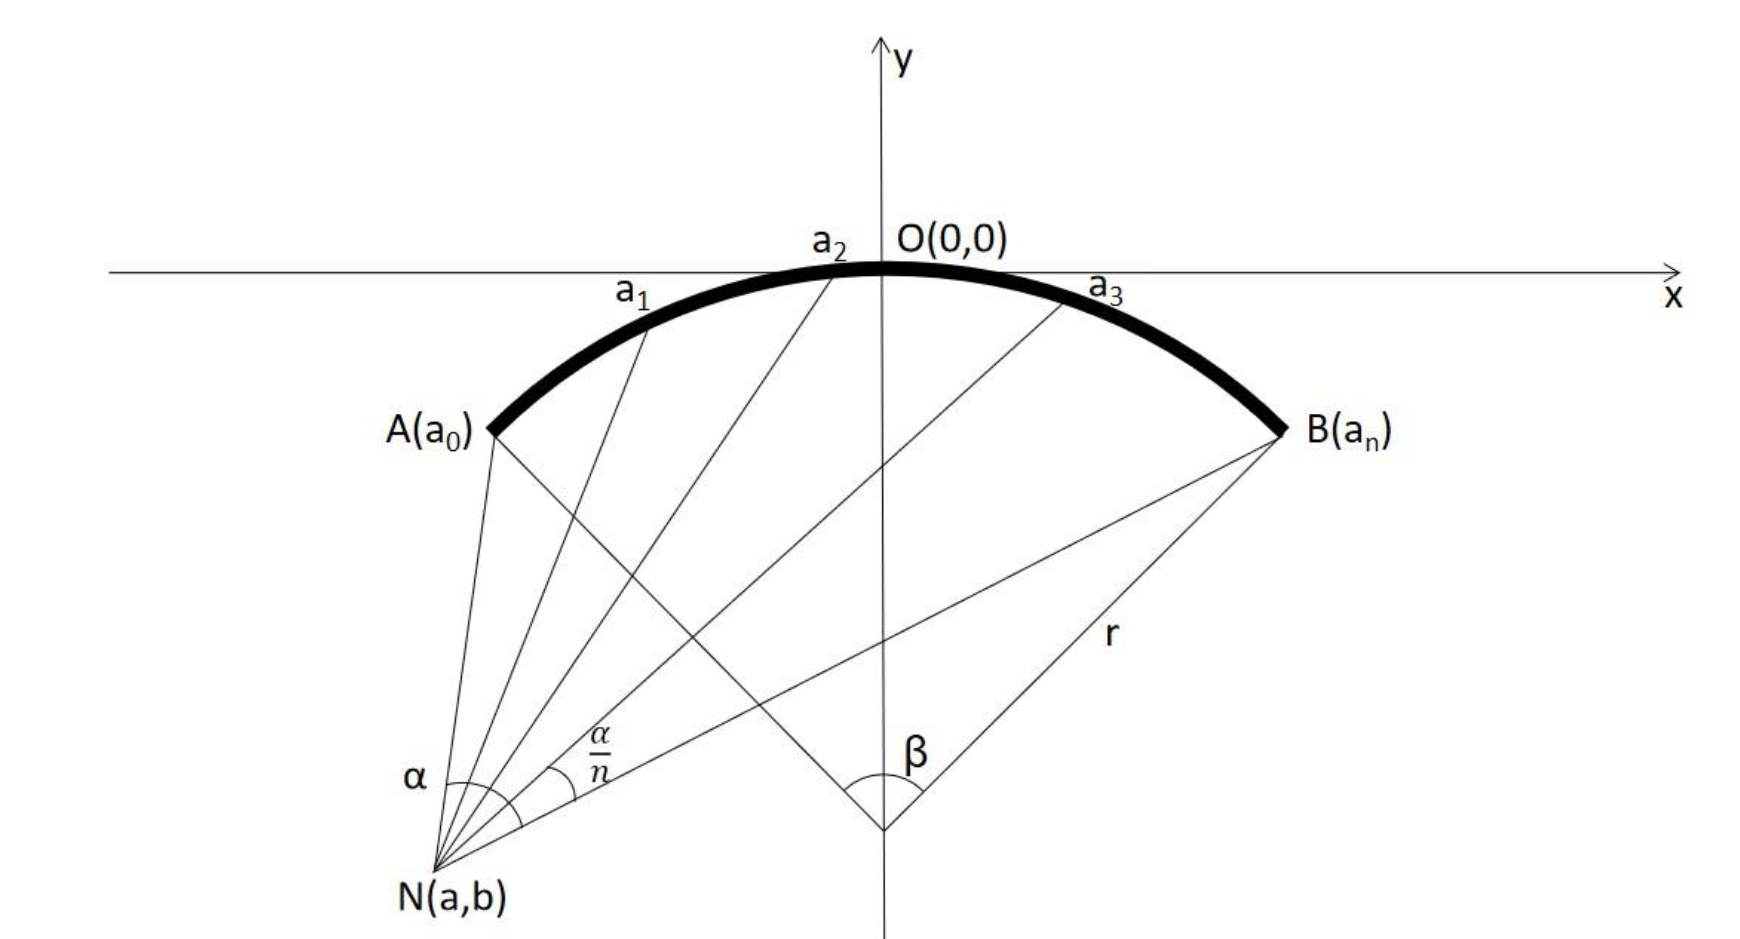
\includegraphics[width=1\textwidth]{figures/Implementation/correction.png}
    \caption{Curved display correction}\label{F:test-a}
\end{figure}

From the three-dimensional coordinates of the user's eye position \( U(x_u, y_u, z_u) \), the three-dimensional coordinates of the screen center \( V(0, 0, \frac{h_s}{2}) \) (where \( h_s \) is the actual screen height) are obtained. Considering only the horizontal visual angle and ignoring the z-coordinate, define the center of the curved screen as the origin \( O(0,0) \), with point \( A \) on the left and point \( B \) on the right of the screen. Suppose the radius of curvature is \( r \), the central angle of the curved screen is \( \beta \), and the user's eye position in the two-dimensional coordinate system is \( N(a, b) \) (where \( a = x_u, b = y_u \)). When the user looks at the screen with coordinates \( V(x_v, y_v) \), the current visual angle \( \alpha \) can be calculated as follows:

\begin{equation}
\alpha = \arccos \left( \frac{\overline{NA} \cdot \overline{NB}}{|\overline{NA}||\overline{NB}|} \right)
\end{equation}

The vectors \( \overline{NA} \) and \( \overline{NB} \) can be expressed as follows:

\begin{equation}
\overline{NA} = (p, q) = \left( -r \sin \frac{\beta}{2} - a, r \cos \frac{\beta}{2} - r - b \right) 
\end{equation}

\begin{equation}
\overline{NB} = (o, q) = \left( r \sin \frac{\beta}{2} - a, r \cos \frac{\beta}{2} - r - b \right)
\end{equation}

Dividing the visual angle \( \alpha \) into \( n \) equal parts, define the intersections of the equal division lines with the screen as \( a_1, a_2, \ldots, a_n \) (where point \( A \) is \( a_0 \), point \( B \) is \( a_n \)). The coordinates of \( a_i \) are noted as \( (x_i, y_i) \):

\begin{align}
    y_i - b &= k_i(x_i - a)
\end{align}
\begin{align}
    x_i^2 + (y_i + r)^2 &= r^2 
\end{align}

From equations (9) and (10), we get:

\begin{align}
y_i = \frac{|k_i| \sqrt{-a^2k_i^2 + 2abk_i + 2ak_ir - b^2 - 2br + k_i^2r^2} - ak_i + b - k_i^2r}{k_i^2 + 1} 
\end{align}
\begin{align}
    x_i = a + \frac{y_i - b}{k_i}
\end{align}

where \( k_i \) is the slope of line \( N a_i \), calculated as follows:

\begin{equation}
k_i = \tan \left( -\frac{i \alpha}{n} + \arctan \left( \frac{q}{p} \right) \right) 
\end{equation}

Once all coordinates \( a_1, a_2, \ldots, a_n \) are obtained, we can calculate the length of each divided segment:

\begin{equation}
a_i a_{i+1} = \left( \arctan \left( \frac{y_i + r}{x_i} \right) - \arctan \left( \frac{y_{i+1} + r}{x_{i+1}} \right) \right) r 
\end{equation}

Thus, the ratio of the deformed segments to the corresponding screen segments can be defined as \( r_n \):

\begin{equation}
r_n = \frac{n a_i a_{i+1}}{\overline{AB}}
\end{equation}

where

\begin{equation}
\overline{AB} = \beta r
\end{equation}

According to the obtained results, the corresponding parts of the deformed screen can be proportionally stretched or shrunk to achieve the desired screen deformation effect.


\section {Experiment and Result}
In this section, we will introduce the experiment setup and results of the proposed system, including measureent accuracy, reaction speed, illusion effects and curved display correction.. In section 5.1, we measuremented the position accuracy before and after the filter. Section 5.2 introduced the reaction speed of the system. Section 5.3 shows the illusion effects from different view angles generated by simulator. Section 5.4 shows the correction effect of curved display.
\subsection{Filter Efficiency}
As section 4.2.2 mentioned, result from pnp solver cannot been used directly, since the result may be noisy and unstable. Figure 12 shows the result from pnp solver before and after kalman filter, with state transition noise covariance matrix $Q_k$ set to:
$$
Q_k = \begin{bmatrix} 0.1 & 0 & 0 & 0 & 0 & 0 \\ 0 & 0.1 & 0 & 0 & 0 & 0 \\ 0 & 0 & 0.1 & 0 & 0 & 0 \\ 0 & 0 & 0 & 0.1 & 0 & 0 \\ 0 & 0 & 0 & 0 & 0.1 & 0 \\ 0 & 0 & 0 & 0 & 0 & 0.1 \end{bmatrix}
$$

and measurement noise covariance matrix $R_k$:
$$
R_k = \begin{bmatrix} 1 & 0 & 0 \\ 0 & 1 & 0 \\ 0 & 0 & 3 \end{bmatrix}
$$

\begin{figure}[htb]
    \centering
    \begin{subfigure}[t]{1\linewidth}
        \centering
        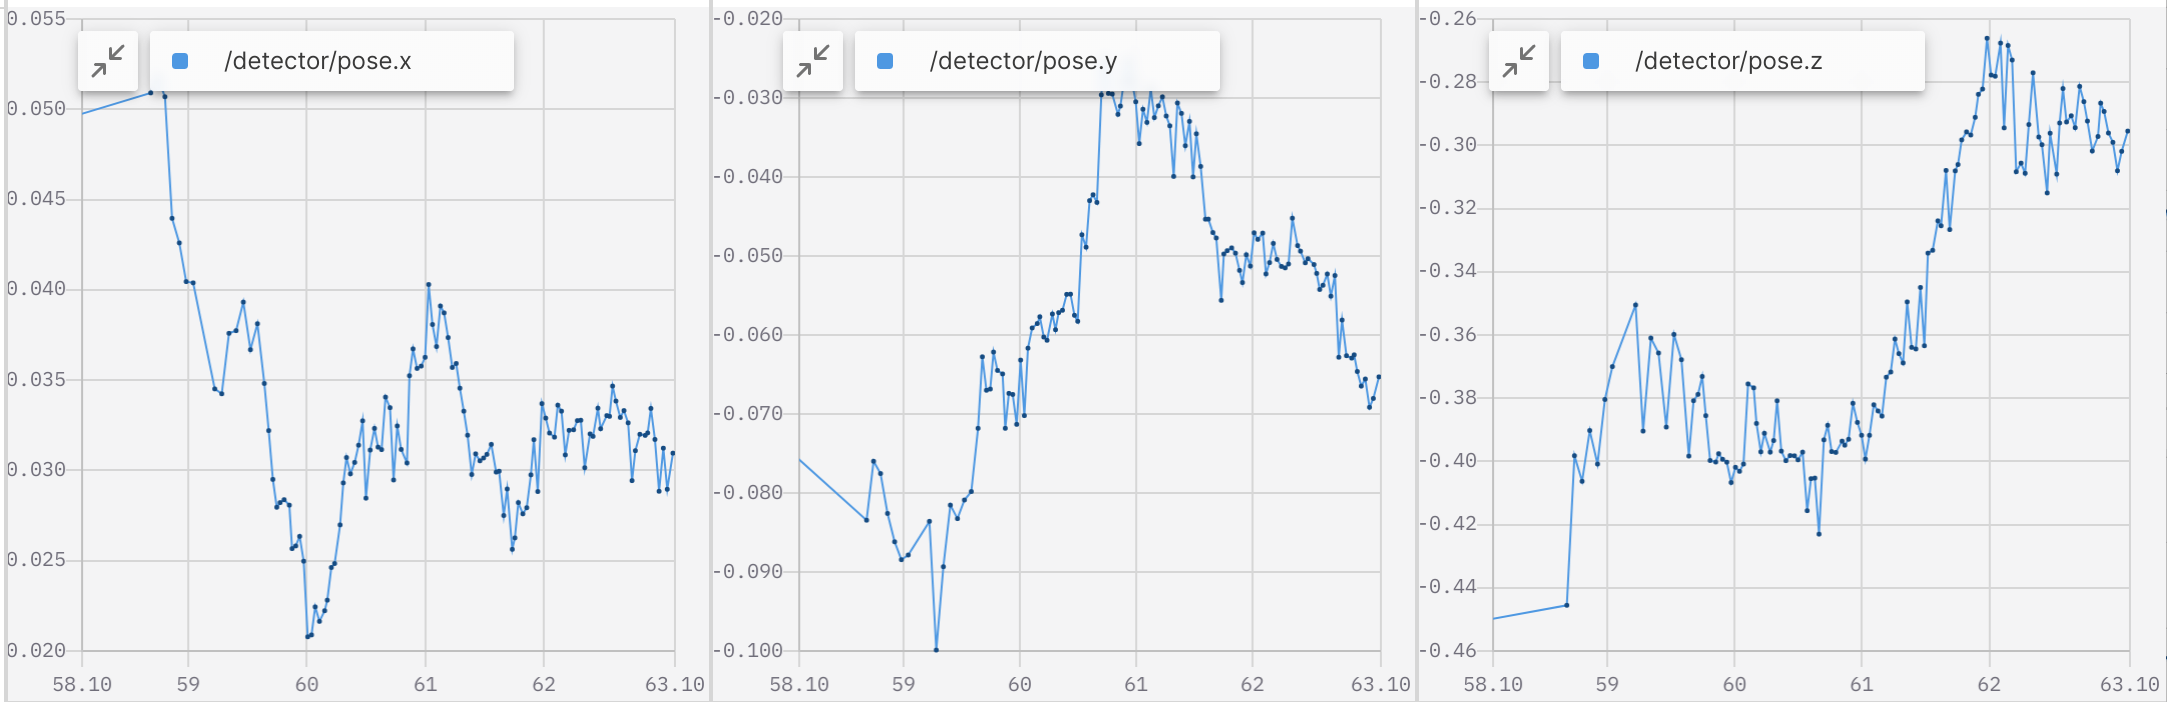
\includegraphics[width=1\textwidth]{figures/Implementation/before_filter.png}
        \caption{Before filter. Vertical axis is face position(m), while horizontal axis is time stamp(s)}\label{F:test-b-sub-a}
    \end{subfigure}
    \begin{subfigure}[t]{1\linewidth}
        \centering
        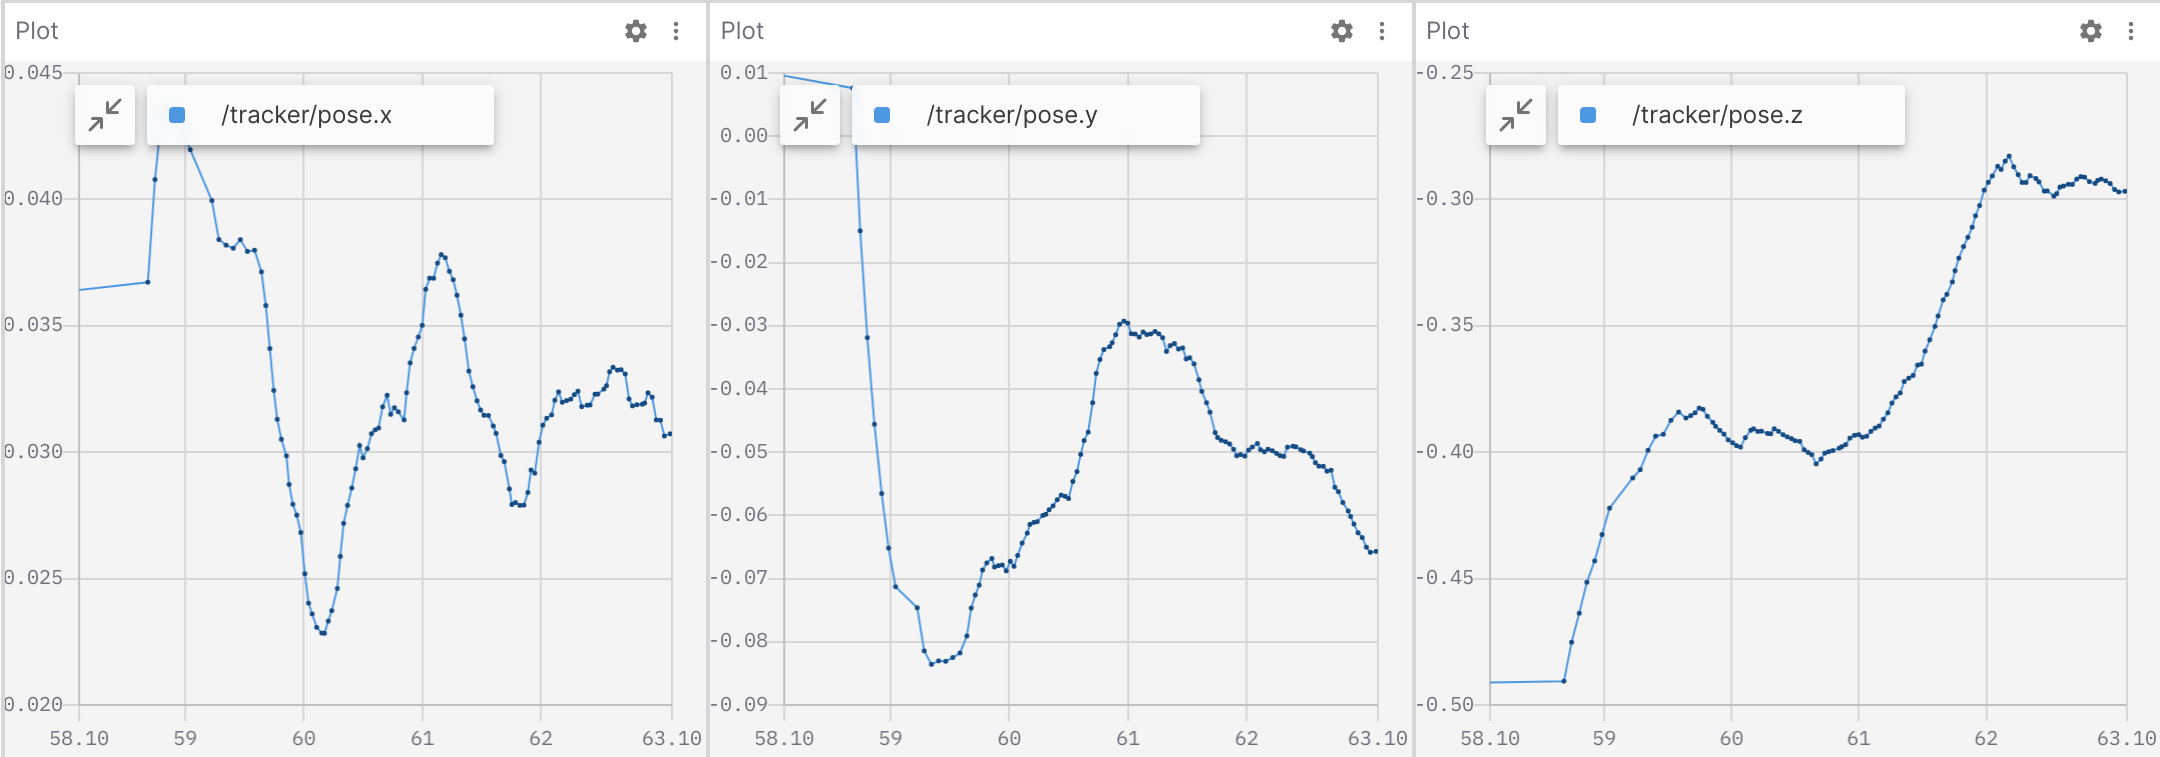
\includegraphics[width=1\textwidth]{figures/Implementation/after_filter.png}
        \caption{After filter. Vertical axis is face position(m), while horizontal axis is time stamp(s)}\label{F:test-b-sub-b}
    \end{subfigure}
    \begin{subfigure}[t]{1\linewidth}
        \centering
        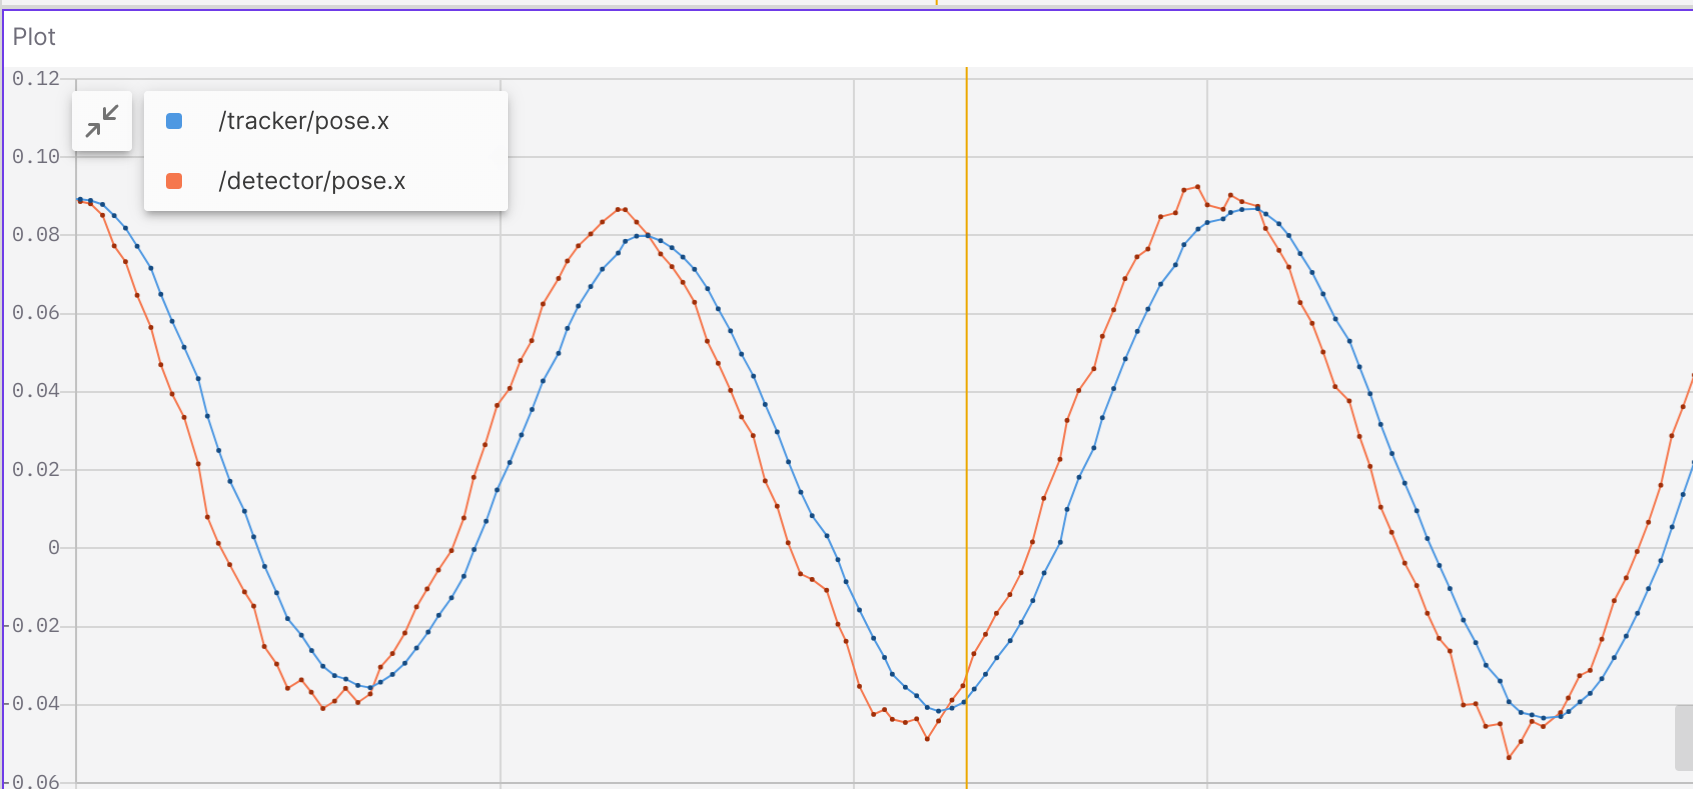
\includegraphics[width=0.9\textwidth]{figures/Implementation/reaction.png}
        \caption{Reaction speed. Yellow is object's movement along x-axis, and blue is result position estimated by filter. Vertical axis is face position(m), while horizontal axis is time stamp(s). Figure shows delay between filter and reality motion is sufficiently short.}\label{F:test-b-sub-b}
    \end{subfigure}
    \caption{}\label{F:test-b}
\end{figure}

Also, reaction speed is also excellent. Figure 17 shows the comparation of measurement and filter result by set object to move along the x-axis.

Motion state estimate is more stable after applying kalman filter. The result is more smooth and less noisy, which is more suitable for 3D display system.
\clearpage

\subsection{Algorithm Performance}
Consider render part usually provided by virtual environment developer, we measured the speed of head tracking and image correction algorithm on a standard Intel i7-12650H/32GB RAM laptop with ROS2 Humble and Ubuntu22.04(kernel version 6.5.0-28). Result is shown in Table 1 and Figure 13. Avg process time of detector is 12ms, head tracking is 3ms, and wrapper is less than 1ms. The algorithm's processing time can be considered to meet the requirements for real-time performance. Moreover, the process can be expedited by employing a more faster face landmark detector and utilizing GPU acceleration.

\begin{figure}
    \centering
    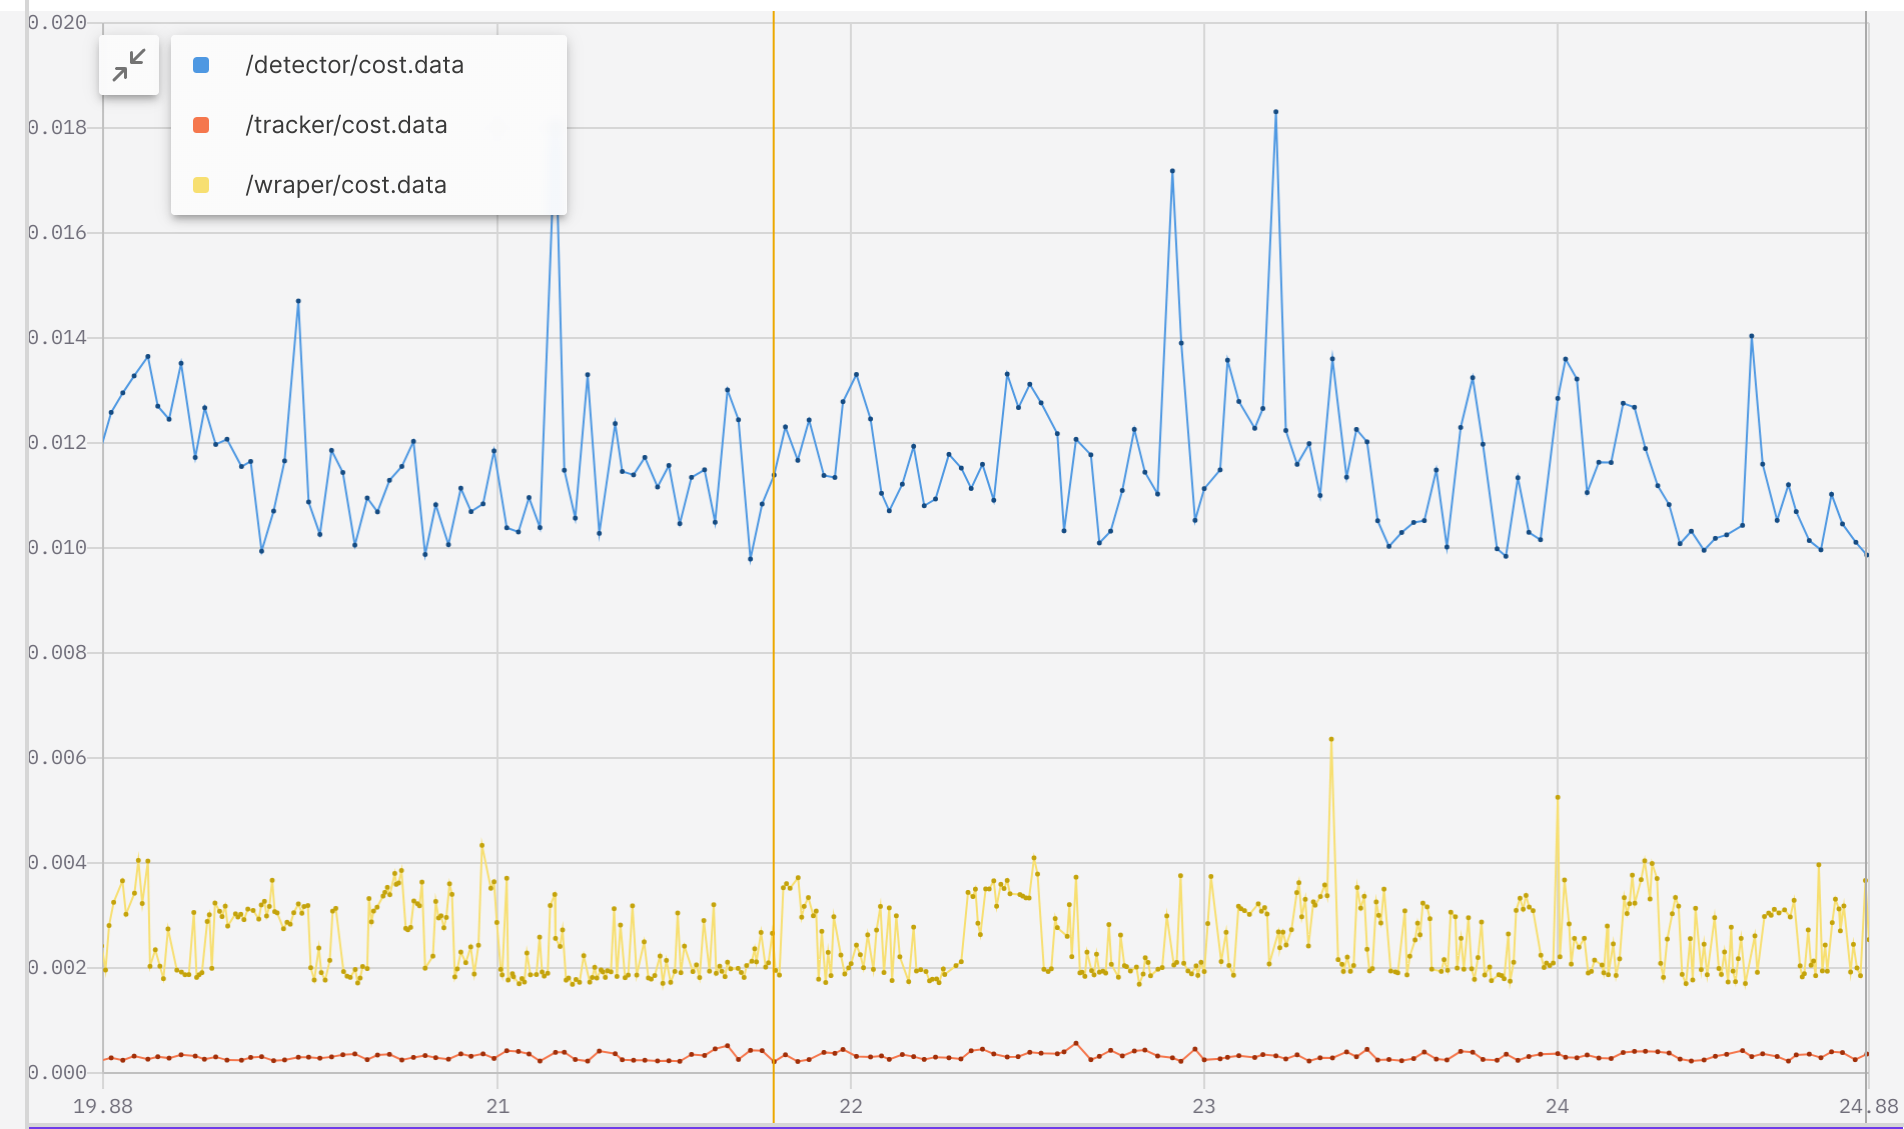
\includegraphics[width=1\textwidth]{figures/Implementation/cost.png}
    \caption{Performance. Horizontal axis is time stamp(s), while vertical axis is algorithm costs (s). The algorithm's processing time can be considered to meet the requirements for real-time performance. }\label{F:test-a}
\end{figure}


\begin{table}[h!]
    \centering
    \begin{tabular}{lc}
        \toprule
        Component     & Avg Time Cost (ms) \\
        \midrule
        Detector      & 12                 \\
        Head-Tracking & 3                  \\
        Wrapper       & < 1                \\
        \bottomrule
    \end{tabular}
    \caption{System cost}
    \label{tab:your_label}
\end{table}

\subsection{Illusion Effects}

As the effectiveness of visual illusions is related to physical factors such as the size of the display, we opted to use a simulator to demonstrate the effects of these illusions more conveniently. In the Unity simulator, the main camera view represents the user's current perspective, and a plane at the center of the field of view shows an image as a display rendering the virtual scene. By binding the main camera, rendering camera, and the user's head position and orientation within the camera coordinate system, we simulated a usage scenario. In this scenario, the effects of visual illusions are very pronounced and exhibit a distinct 3D effect. Figure 14 illustrates the resultant illusion effect. As the user’s head moves, the objects' positions on the screen dynamically adjust accordingly. The plane functions as a virtual display, simulating the content perceived by the user.

Additionally, we assessed our correction algorithm using sample images. Figure 15 presents the outcome of this correction process. The initial image is distorted by the curvature of the screen, but our correction algorithm successfully adjusts the image to align with the screen's viewing angle.

\begin{figure}
    \centering
    \begin{subfigure}[t]{0.45\linewidth}
        \centering
        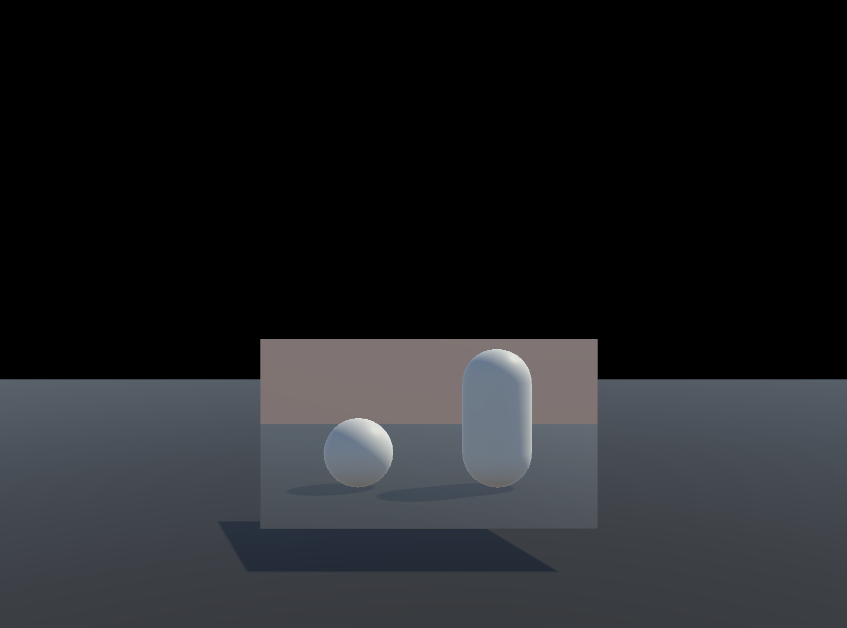
\includegraphics[width=1\textwidth]{figures/Implementation/illusion_1.png}
    \end{subfigure}
    \begin{subfigure}[t]{0.45\linewidth}
        \centering
        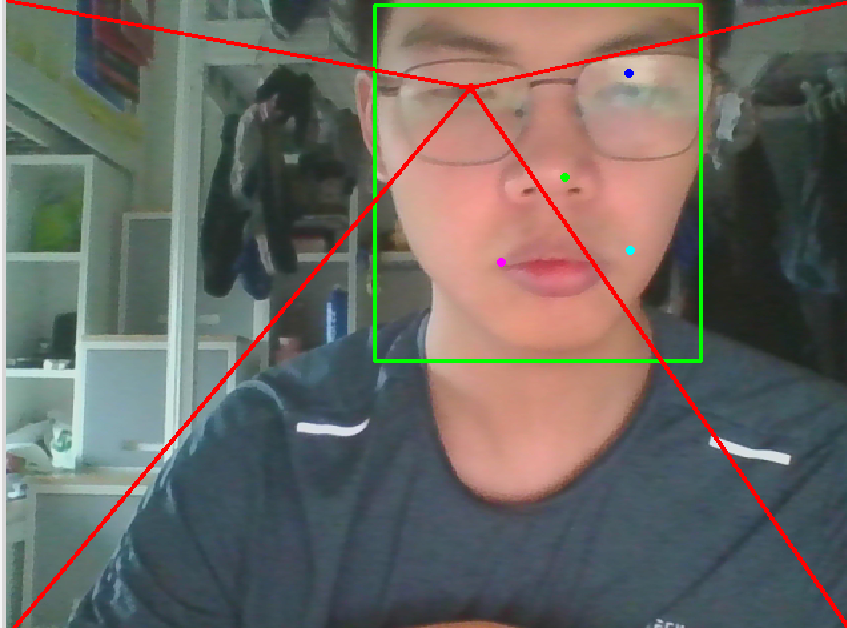
\includegraphics[width=1\textwidth]{figures/Implementation/illusion_1_face.png}
    \end{subfigure}
    \begin{subfigure}[t]{0.45\linewidth}
        \centering
        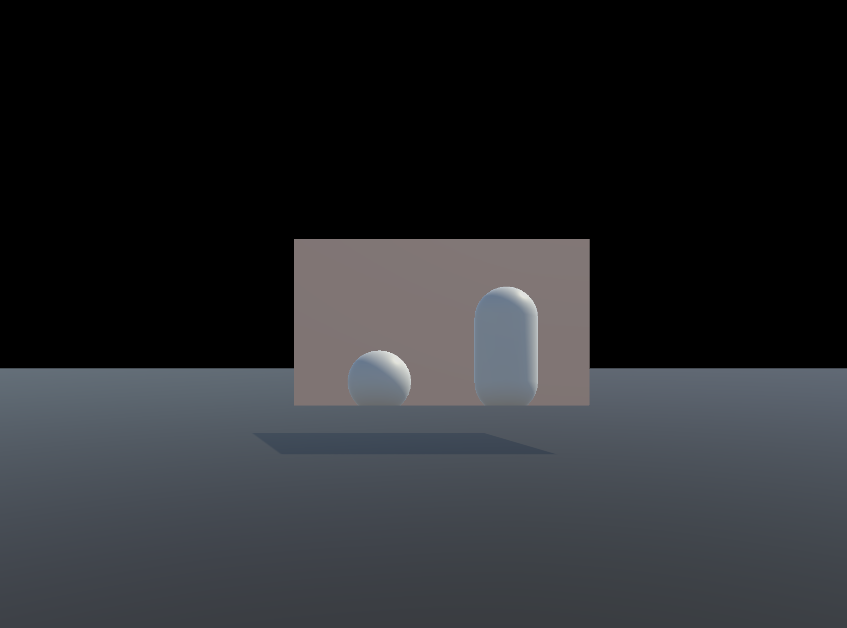
\includegraphics[width=1\textwidth]{figures/Implementation/illusion_2.png}
    \end{subfigure}
    \begin{subfigure}[t]{0.45\linewidth}
        \centering
        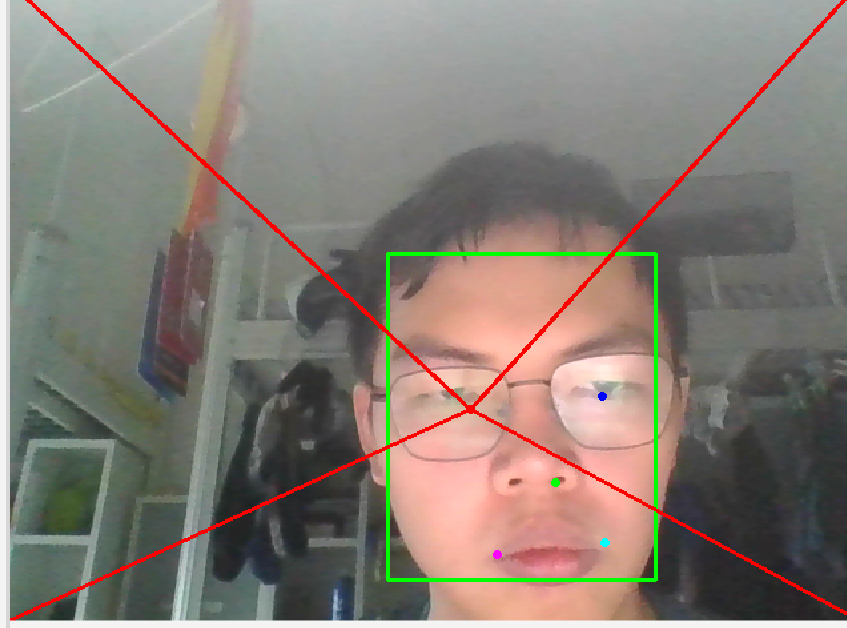
\includegraphics[width=1\textwidth]{figures/Implementation/illusion_2_face.png}
    \end{subfigure}
    \begin{subfigure}[t]{0.45\linewidth}
        \centering
        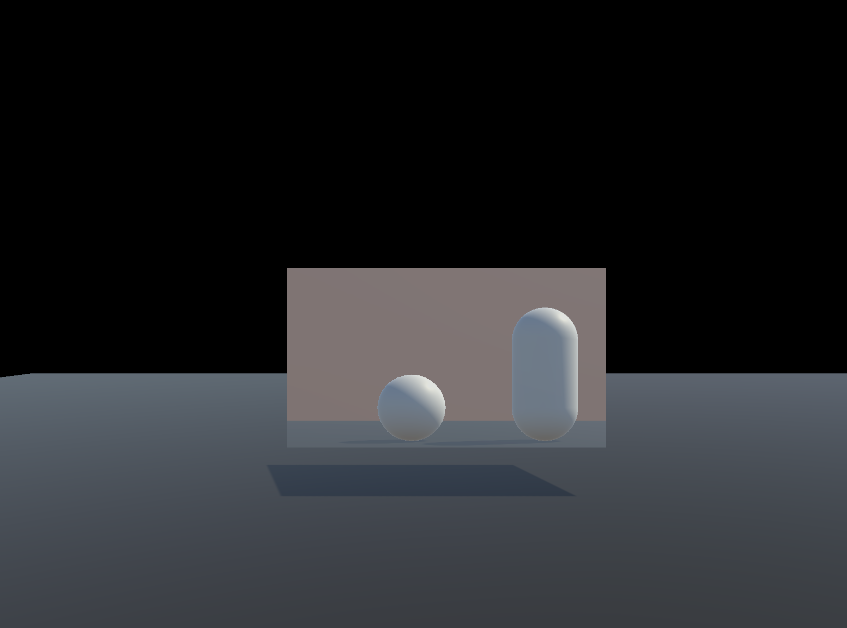
\includegraphics[width=1\textwidth]{figures/Implementation/illusion_3.png}
    \end{subfigure}
    \begin{subfigure}[t]{0.45\linewidth}
        \centering
        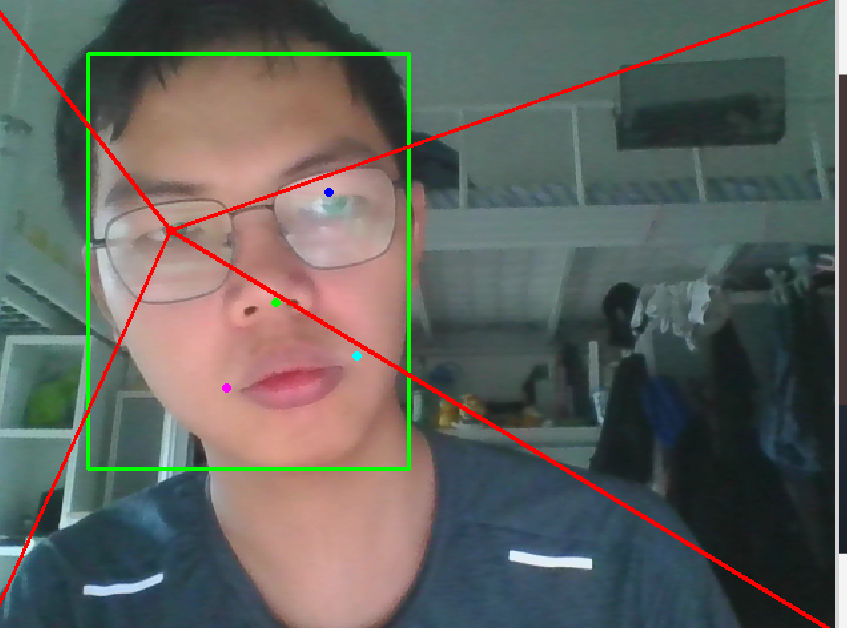
\includegraphics[width=1\textwidth]{figures/Implementation/illusion_3_face.png}
    \end{subfigure}
    \caption{Illusion effects in simulation environment. Camera view represents the user's current perspective, and a plane at the center of the field of view shows an image as a display rendering the virtual scene. Illusion is obvious in simulation environment.}\label{F:test-b}
\end{figure}

\begin{figure}
    \centering
    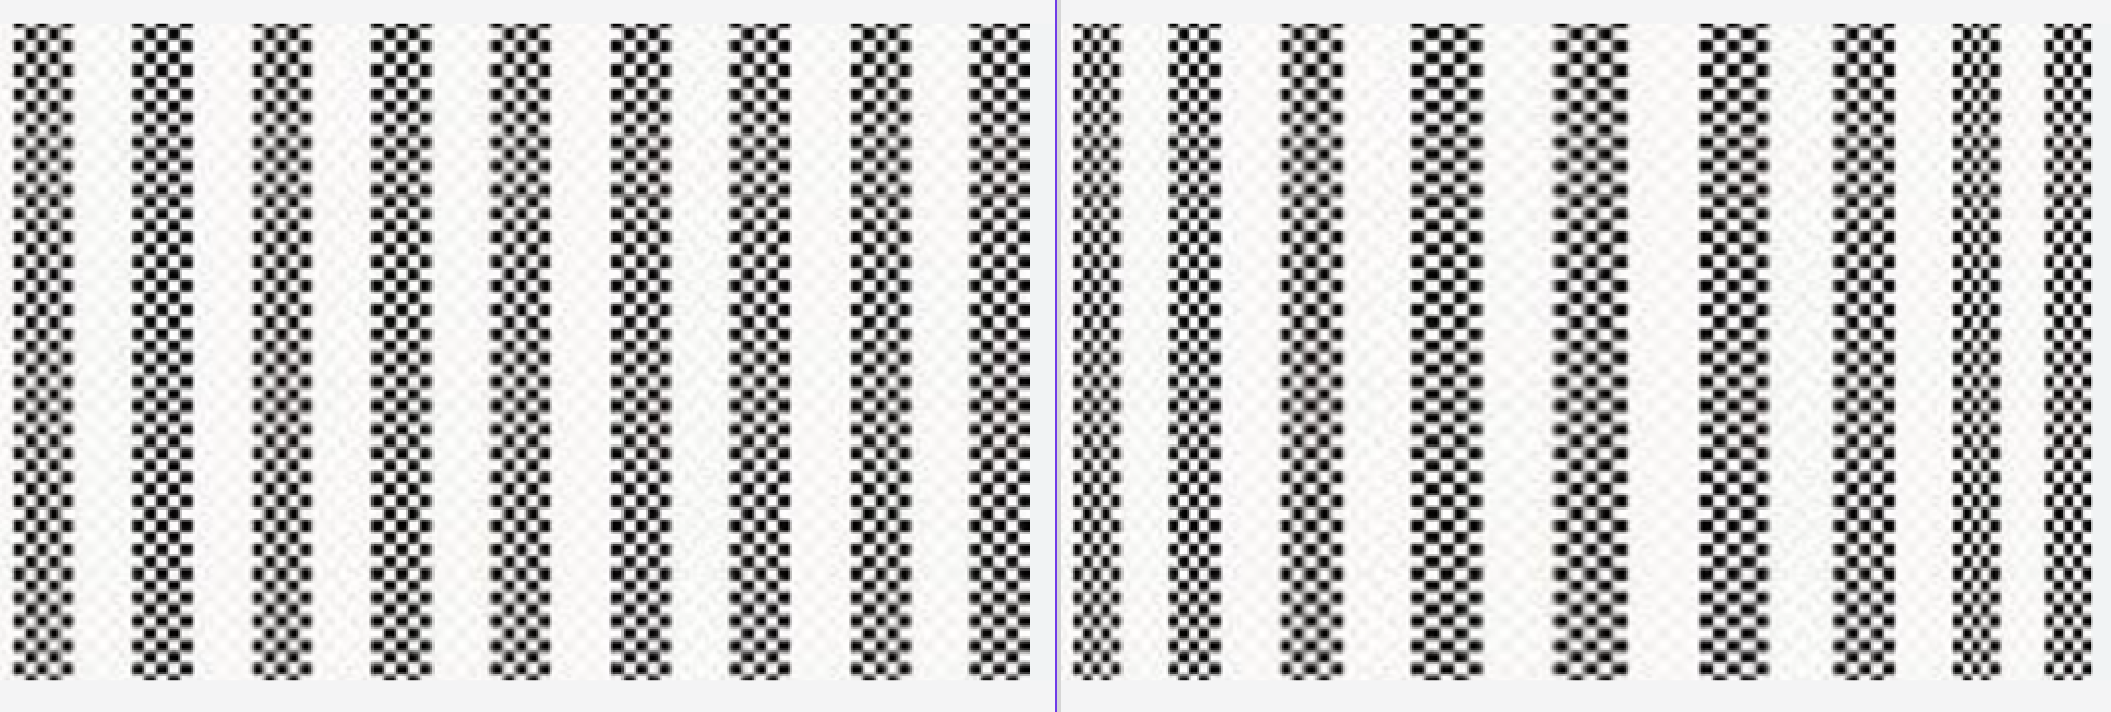
\includegraphics[width=1\textwidth]{figures/Implementation/correction_example.png}
    \caption{Correction on sample}\label{F:test-a}
\end{figure}
\clearpage